
\documentclass[border={0pt 0pt 0pt 0pt}]{standalone}
\usepackage{tikz-cd,tikz-3dplot} 
\usetikzlibrary{calc,intersections,through,backgrounds,decorations.pathmorphing, decorations.shapes,decorations.markings}
%include other needed packages here   
\begin{document}
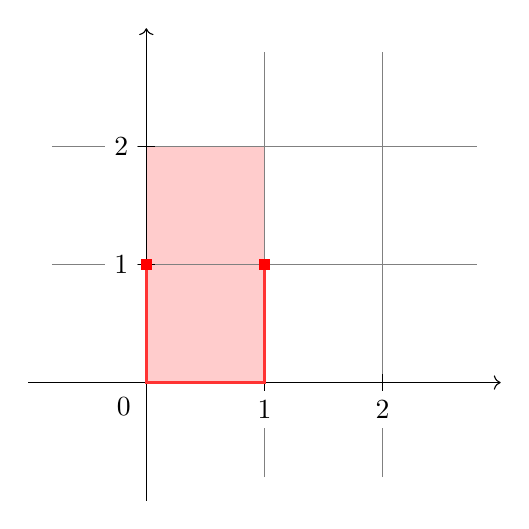
\begin{tikzpicture}[scale=3]



\fill[red!20!white] (0,0) -- (0.5,0) -- (0.5,1) -- (0,1) -- (0,0);

\draw[step=.5cm,gray,very thin] (-0.4,-0.4) grid (1.4,1.4);
\draw[->] (-0.5,0) -- (1.5,0);
\draw[->] (0,-0.5) -- (0,1.5);
\foreach \x/\xtext in {0.5/1,1/2}
\draw (\x cm,1pt) -- (\x cm,-1pt) node[anchor=north,fill=white] {$\xtext$};
\foreach \y/\ytext in {0.5/1,1/2}
\draw (1pt,\y cm) -- (-1pt,\y cm) node[anchor=east,fill=white] {$\ytext$};
\draw (-0.7pt,-0.7pt)  node[anchor=north east,fill=white] {0};

\draw[red!80!white,very thick] (0,0.5) -- (0,0) -- (0.5,0) -- (0.5,0.5);
\node [fill=red,inner sep=2pt] at (0,0.5) {};
\node [fill=red,inner sep=2pt] at (0.5,0.5) {};
\end{tikzpicture}
\end{document}